% !TeX spellcheck = en-US, de-DE
% !TeX encoding = UTF-8 Unicode
\documentclass[169,9pt]{beamer}

\usetheme[
    %% Language, passed to babel/polyglossia
    english, % or (n)german
    localization=babel, % or polyglossia or none
    biblatexbackend=bibtex8, % or biber or bibtex (7-bit)
    %
    %% Imports
    tikz, % import tikz and commonly used packages
    % minted, % import minted and set-up associated environments
    % cleveref, % import cleveref and set-up some names
    %
    %% LuaLaTeX
    % The three following options require LuaLaTeX, which may increase compilation times substantially.
    % localization=polyglossia, % This replaces babel
    % libertine, % Use Linux Libertine/Biolinum as roman/sans serif font
    % firacode, % Use Fira Code as monospaced font
    %
    %% Colors (GU corporate colors are always available)
    ttlabcolors, % TTLab colors
    % materialcolors, % Material default colorscheme colors
    % alphabetcolors, % Alphabet color scheme, REQUIRES CITATION
    % greenarmytagecolors, % Green-Armytage color scheme, REQUIRES CITATION
    %
    %% Layout options
    titlemargin=0.1\paperwidth, % the size of margins left and right of the title
    titleheight=0.4\paperheight, % the hight of the beamercolorbox containing title and subtitle
    titledepth=0\paperheight, % the depth of the beamercolorbox containing title and subtitle
    % centertitle, % center the title and subtitle
    sectionheight=0.5\paperheight, % the height of the section title box section/subsection frame
    frametitlemargin=0.3cm, % the size of the margin left of each frame title and subtitle
    framefootermargin=0.3cm, % the size of the margins left and right in the footline
    logo=images/TTLogo-2.pdf, % can be PDF or any image, is scaled to logowidth
    logowidth=0.4\paperwidth, % you may need to scale your logo to fit the title page
    % centerlogo, % center the logo on the title page
    % nologo, % disable the logo on the title page
    % nonavigation, % disable the navigation in the footline
]{goethe}

\setbeamertemplate{navigation symbols}{} %hides navigation buttons at bottom
\setbeamercovered{transparent}

%%%%%%%%%%%%%%%%%%%%%%%%
% Title, Authors, etc. %
%%%%%%%%%%%%%%%%%%%%%%%%
% Authors and titles are wrapped in a tblr environment

% Title and sub-title can contain \\
\title[Dualität]{Dualität} % TODO
\subtitle[]{Welche grundlegenden Unterschiede und
Gemeinsamkeiten bestehen zwischen
künstlichen und menschlichen
Informationssystemen?} % TODO

% Authors in "middle" alignment
% Separate multiple authors on the same line with \and
% Use \And to put authors on a separate line
\author[X. Wang]{Xinran Wang}

% Date in "footer" alignment, bottom right
\date{\today} % TODO

%%%%%%%%%%%%
% Footline %
%%%%%%%%%%%%
% Uncomment and change the following lines to change the footline
% \makeatletter%
% \setbeamertemplate{footline separator}{~--~}
% \setbeamertemplate{footline content}{%
%     \let\hyperlink\@secondoftwo%
%     \insertshorttitle\usebeamertemplate{footline separator}\insertshortsubtitle%
% }
% \makeatother%

%%%%%%%%%%%%%%%%
% Bibliography %
%%%%%%%%%%%%%%%%
\usepackage[backend=biber]{biblatex}
\usepackage{graphicx}
\usepackage{algorithm}
\usepackage{algpseudocode}
\usepackage{amsmath}
\usepackage{amsfonts}
% Note, that we cannot import the whole ACL anthology using biber, as it takes forever to run.
% Instead, we can fall back to the bibtex8 backend by passing biblatexbackend=bibtex8 as an.
% Add the bibliography files using:
\addbibresource{quellen.bib}

%%%%%%%%%%%%
% Document %
%%%%%%%%%%%%
\begin{document}

\maketitle

\section{Was ist ein Informationssystem?}\sectionFrame

\begin{frame}{Was ist ein Informationssystem?}
Ein strukturiertes System : Sammlung, Speicherung, Verarbeitung und Bereitstellung von Informationen.
    \begin{itemize}
        \item Gemeinsamkeiten
              \begin{itemize}
                  \item<1-> Informationverarbeitung
                  \item<1-> Speicherung von Informationen
                  \item<1-> Kommunikation
                  \item<1-> Anpassung
              \end{itemize}
    \end{itemize}
    \begin{itemize}
        \item<2-> Unterschiede
            \begin{columns}
                \begin{column}{0.45\textwidth}
                    \textbf{KI}
                        \begin{itemize}
                            \item Hardware und Software
                            \item Durch Maschinelles Lernen und KI-Algorithmen
                            \item Große Datenmenge \(\Rightarrow\) Schneller
                            \item In ihrer Flexibilität und Kreativität begrenzt
                            \item Große Mengen an Daten schnell verarbeiten
                        \end{itemize}
                \end{column}
                \begin{column}{0.45\textwidth}
                    \textbf{Menschen}
                        \begin{itemize}
                            \item Das menschliche Gehirn
                            \item Durch Erfahrung, Beobachtung und Interaktion => langsamer, komplexer
                            \item Flexibel und kreativ
                            \item komplexe Aufgaben mit relativ wenig Energie bewältigen
                        \end{itemize}
                \end{column}
            \end{columns}
    \end{itemize}
\end{frame}

\section{KI kann nicht die Kreativität des Menschen haben}\sectionFrame[show subsections]
\subsection{Beethoven's Ninth and AI's Tenth}

\begin{frame}{KI kann nicht die Kreativität des Menschen haben}{Was für Kreativität notwendig ist, aber bei KI fehlt?(Menschliche Kreativität)}
    \begin{itemize}
            \item<1-> Intrinsische Motivation
                \begin{itemize}
                    \item<1-> Fehlende Bewusstheit
                    \item<1-> Programmiert von Menschen
                    \item<1-> Keine eigenen Bedürfnisse oder Wünsche
                    \item<1-> Fehlende Emotionen 
                \end{itemize}
            \item<2-> Authentizität
            \begin{itemize}
                    \item<2-> Sich selbst akzeptiert
                    \item<2-> Nicht sich selbst übermäßig zu überprüfen oder ständig sein Verhalten zu filtern
                    \item<2-> Einschränkung durch menschliche Programmierung und Anweisung
                \end{itemize}
            \item<3-> Problem finding
                \begin{itemize}
                    \item<3-> Problemerkennung
                    \item<3-> Problemdefinition
                    \item<3-> Problemformulierung
                    \item<3-> Problemkonstruktion
                    \item<3-> Ein Computer könnte gute Probleme finden, müsste aber angewiesen werden, nach ihnen zu suchen.
                \end{itemize}            
    \end{itemize}
\end{frame}


\begin{frame}{KI kann nicht die Kreativität des Menschen haben}{Beethoven's Ninth
and AI's Tenth}
    \begin{itemize}
        \item 1827: Der Komponist Ludwig van Beethoven starb
        \item 2021: Ein Team von Informatikern und Musikern vervollständigen mittels KI die 10.Symphonie
        \item Vergleich von 2 Kompositionen
            \begin{itemize}
                \item Das KI-Modell erfasst einige Merkmale der menschlichen Kreativität
                \item Weniger für: 
                    \begin{itemize}
                        \item 1. Nichtlineares Denken
                        \item 2. Komtextgesteuerte Entscheidungsfindung
                    \end{itemize}
            \end{itemize}
    \end{itemize}
\end{frame}

\begin{frame}{KI kann nicht die Kreativität des Menschen haben}{Beethoven's Ninth and AI's Tenth}
\begin{figure}[h]
    \centering
    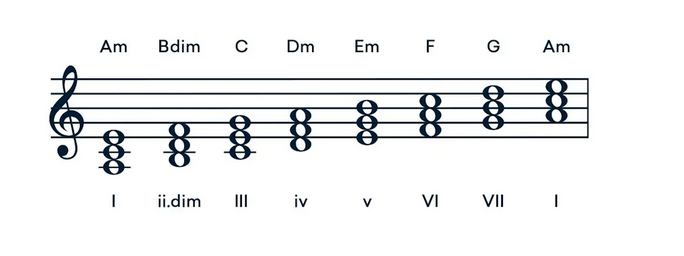
\includegraphics[width=0.7\textwidth]{Bildschirmfoto vom 2024-07-21 11-21-32.png}
    \caption{\smaller \smaller \smaller \smaller https://blog.landr.com/de/dur-akkorde/}
    \label{fig:my_label}
\end{figure}
\begin{algorithm}[H]
    \caption{Definition von Akkorden}
    \begin{algorithmic}[1]
    \State \textbf{Define} CHORDS as:
    \State \{ "C": ["C", "E", "G"], \\"Dm": ["D", "F", "A"], \\"Em": ["E", "G", "B"],\\ "F": ["F", "A", "C"], \\"G": ["G", "B", "D"], \\"Am": ["A", "C", "E"], \\"Bdim": ["B", "D", "F"] \}
    \State    
    \end{algorithmic}
    \end{algorithm}
\end{frame}

\begin{frame}{KI kann nicht die Kreativität des Menschen haben}{Beethoven's Ninth and AI's Tenth}
\begin{algorithm}[H]
    \caption{Definition von Akkordprogressionen}
    \begin{algorithmic}[1]
    \State \textbf{Define} CHORD\_PROGRESSIONS as:
    \State \{ ["C", "F", "G", "C"],
    \State ["C", "G", "Am", "F"],
    \State ["C", "Em", "F", "G"],
    \State ["Am", "F", "C", "G"] \}
    \State
    \end{algorithmic}
\end{algorithm}
\end{frame}

\begin{frame}{KI kann nicht die Kreativität des Menschen haben}{Beethoven's Ninth and AI's Tenth}
\begin{algorithm}[H]
\caption{Zufällige Auswahl einer Akkordprogression}
\begin{algorithmic}[1]
\State \textbf{function} \textsc{RandomChoice}(list)
    \State \quad \textbf{return} a random element from list
\EndFunction
\State chosen\_progression = \textsc{RandomChoice}(CHORD\_PROGRESSIONS)
\State
\end{algorithmic}
\end{algorithm}
\end{frame}

\begin{frame}{KI kann nicht die Kreativität des Menschen haben}{Beethoven's Ninth and AI's Tenth}\begin{algorithm}[H]
\caption{Erzeugung einer Akkordprogression}
\begin{algorithmic}[1]
\State \textbf{function} \textsc{GenerateChordProgression}(progression)
    \State \quad chord\_progression = []
    \For {each chord in progression}
        \State \quad \quad \textbf{add} CHORDS[chord] to chord\_progression
    \EndFor
    \State \quad \textbf{return} chord\_progression
\EndFunction
\end{algorithmic}
\end{algorithm}
\end{frame}

\begin{frame}{KI kann nicht die Kreativität des Menschen haben}{Beethoven's Ninth and AI's Tenth}\begin{algorithm}[H]
\caption{Erzeugung einer Melodie}
\begin{algorithmic}[1]
\State \textbf{function} \textsc{GenerateMelody}(chord\_progression)
    \State \quad melody = []
    \For {each chord in chord\_progression}
        \State \quad \quad melody\_note = \textsc{RandomChoice}(chord)
        \State \quad \quad \textbf{add} melody\_note to melody
    \EndFor
    \State \quad \textbf{return} melody
\EndFunction
\end{algorithmic}
\end{algorithm}
\end{frame}

\begin{frame}{KI kann nicht die Kreativität des Menschen haben}{Beethoven's Ninth and AI's Tenth}\begin{algorithm}[H]
\caption{Hauptprogramm}
\begin{algorithmic}[1]
\State chord\_progression = \textsc{GenerateChordProgression}(chosen\_progression)
\State melody = \textsc{GenerateMelody}(chord\_progression)
\State \textbf{print} "Chord Progression:", chosen\_progression
\State \textbf{print} "Melody:", melody
\State
\end{algorithmic}
\end{algorithm}
\end{frame}


\begin{frame}{KI kann nicht die Kreativität des Menschen haben}{Beethoven's Ninth
and AI's Tenth}
\textbf{Lineares Denken}: Geradlinigen und sequenziellen Schritten\\
\textbf{Nichtlineares Denken}: Assoziationen, Intuition und nicht-lineare Verknüpfungen
\begin{figure}[h]
    \centering
    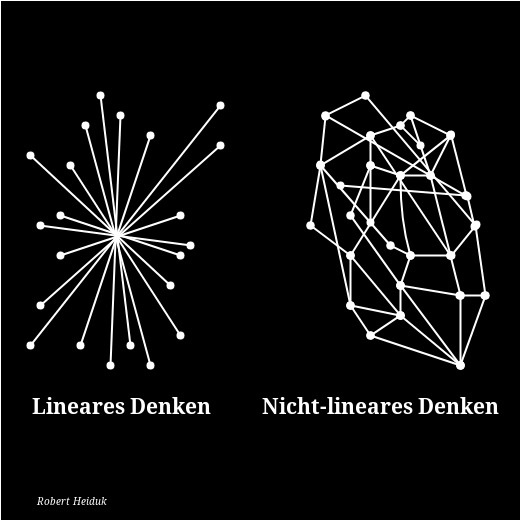
\includegraphics[width=0.5\textwidth]{images/non-linear-1.jpg}
    \caption{\smaller \smaller https://blog.eisenklinik.de/2019/09/26/hat-klassische-trainingssteuerung-ausgedient/}
    \label{fig:my_label}
\end{figure}
\end{frame}



\begin{frame}{KI kann nicht die Kreativität des Menschen haben}{Beethoven's Ninth
and AI's Tenth}
    \begin{columns}
                \begin{column}{0.45\textwidth}
                    \textbf{KI}
                        \begin{itemize}
                            \item Schrittweise in einer festen Reihenfolge
                            \item Zusammengesetztes Werk
                            \item Pixelierter Schöpfungsprozess
                            \item Wortwörtliche Wiedergabe des Themas
                            \item Häufig zu lange in einer Tonart verweilen
                            \vspace{\baselineskip} 
                            \item \textbf{Überraschung:} Orgel
                            \item \textbf{Beitrittsmethode:}unvermittelt
                        \end{itemize}
                \end{column}
                \begin{column}{0.45\textwidth}
                    \textbf{Beethoven}
                        \begin{itemize}
                            \item Außerhalb einer strikten zeitlichen Reihenfolge komponieren kann.
                            \item Die Melodie von Ode an die Freude wurde zuerst komposiert.
                            \item Der Klang des Orchesters wuede abgelehnt und leitete damit den Chorabschnitt ein.
                            \vspace{\baselineskip}
                            \item \textbf{Überraschung:}Die Sängern hinzufügen
                            \item \textbf{Beitrittsmethode:}Eine musikalische Infrastruktur ist zu schaffen
                        \end{itemize}
                \end{column}
            \end{columns}    
\end{frame}

\begin{frame}{KI kann nicht die Kreativität des Menschen haben}{Beethoven's Ninth and AI's Tenth}
\begin{columns}
    \begin{column}{0.45\textwidth}
        \begin{figure}[h]
            \centering
            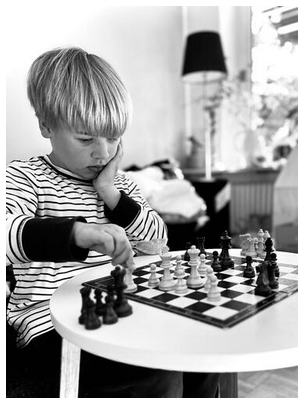
\includegraphics[width=1.0\textwidth]{Bildschirmfoto vom 2024-07-19 19-31-37.png}
            \caption{\smaller \smaller \smaller \smaller \smaller https://www.photocase.de/fotos/5344695-der-meister-und-sein-endgegner-kind-spielt-gegen-sich-selbst-schach-photocase-stock-foto \newline Letzter Zugriff: 28.Juni (Screenshot vom 19.Juli 2024, 15:48 Uhr)}
            \label{fig:my_label}
        \end{figure}
    \end{column}
    \begin{column}{0.45\textwidth}
        \textbf{Kontextgesteuerte Entscheidungsfindung:} Berücksichtigung von Umgebung und Situation
    \end{column}
\end{columns}
\end{frame}

\begin{frame}{KI kann nicht die Kreativität des Menschen haben}{Beethoven's Ninth and AI's Tenth}
    \begin{figure}[h]
    \centering
    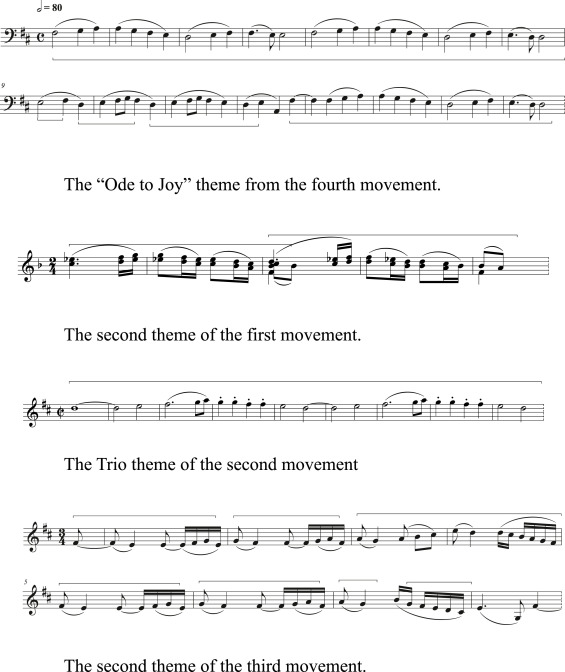
\includegraphics[width=0.5\textwidth]{BethovenNoten.jpg}
    \caption{\smaller \smaller https://www.sciencedirect.com/science/article/pii/S2713374523000274}
    \label{fig:my_label}
\end{figure}
\end{frame}

\section{Die Stärke der KI}\sectionFrame[show subsections]
\subsection{KI und Kontrolle des Covid-19-Coronavirus}

\begin{frame}{Die Stärke der KI}{KI und Kontrolle des Covid-19-Coronavirus}
Anfang 2020: die Viruspandamie\\
KI als Instrument zur Unterstützung gegen die Viruspandemie\\
\begin{itemize}
    \item Schnelle Identifizierung und Frühwarnung
    \item Beschleunigung von Forschung und Impfstoffentwicklung
    \item Erhöhung der Diagnosegeschwindigkeit und –genauigkeit
    \item Förderung des Wissensaustauschs
\end{itemize}
\end{frame}

\begin{frame}{Die Stärke der KI}{KI und Kontrolle des Covid-19-Coronavirus}
Vorteile im Vergleich zum Menschen
\begin{itemize}
    \item Geschwindigkeit und Effizienz
    \item Präzision und Konsistenz
    \item Verarbeitung großer Datenmengen
    \item Vorhersage und Frühwarnung
    \item Automatisierung und Rund-um-
die-Uhr-Arbeit
\end{itemize}
\end{frame}

\section{Zusammenarbeit zwischen Mensch und KI}\sectionFrame[show subsections]
\subsection{Historischen Lernen mit Virtual Reality}

\begin{frame}{Zusammenarbeit zwischen Mensch und KI}{AR und VR in Bildungsarbeit}
Rome Reborn
\begin{figure}[h]
    \centering
    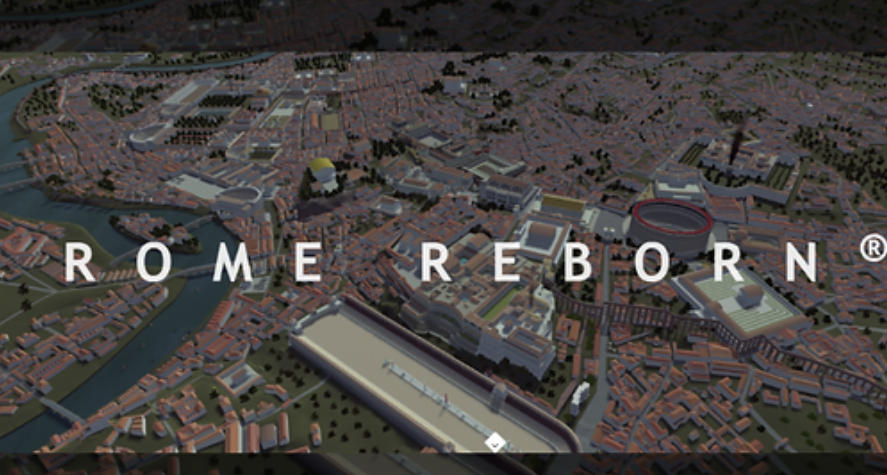
\includegraphics[width=1.0\textwidth]{RomeReburn1.png}
    \caption{\smaller \smaller https://www.avalon-virtual.be/product-page/rome-reborn}
    \label{fig:my_label}
\end{figure}
\end{frame}

\begin{frame}{Zusammenarbeit zwischen Mensch und KI}{AR und VR in Bildungsarbeit}
Rome Reborn
\begin{figure}[h]
    \centering
    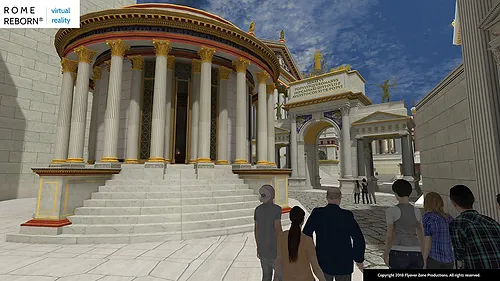
\includegraphics[width=1.0\textwidth]{Romereborn2.png}
    \caption{\smaller \smaller https://www.avalon-virtual.be/product-page/rome-reborn}
    \label{fig:my_label}
\end{figure}
\end{frame}

\begin{frame}{Zusammenarbeit zwischen Mensch und KI}{AR und VR in Bildungsarbeit}
Rome Reborn
\begin{figure}[h]
    \centering
    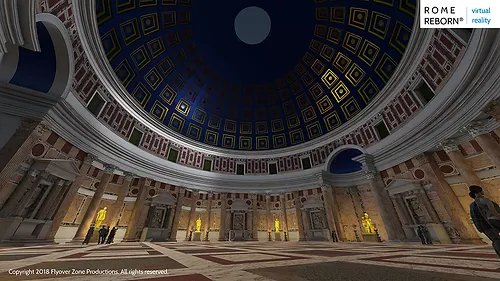
\includegraphics[width=1.0\textwidth]{RomeReborn3.png}
    \caption{\smaller \smaller https://www.avalon-virtual.be/product-page/rome-reborn}
    \label{fig:my_label}
\end{figure}
\end{frame}

\begin{frame}{Zusammenarbeit zwischen Mensch und KI}{AR und VR in Bildungsarbeit}
WDR AR 1933-1945
\begin{figure}[h]
    \centering
    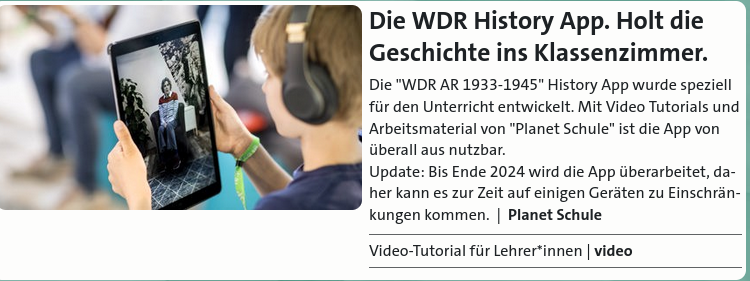
\includegraphics[width=1.0\textwidth]{Bildschirmfoto vom 2024-07-19 20-54-04.png}
    \caption{\smaller \smaller https://www1.wdr.de/fernsehen/unterwegs-im-westen/ar-app/index.html \newline Letzter Zugriff: 19.Juli (Screenshot vom 19.Juli 2024, 20:54 Uhr)}
    \label{fig:my_label}
\end{figure}
\end{frame}

\begin{frame}{Zusammenarbeit zwischen Mensch und KI}{AR und VR in Bildungsarbeit}
\begin{columns}
                \begin{column}{0.45\textwidth}
                    \textbf{Virtual-Reality-Unterricht}
                        \begin{itemize}
                            \item Eintauchen in das Lernerlebnis
                            \item Stärkung der emotionalen Verbindung und des Verständnisses
                            \item Multisensorisches Lernen
                            \item Zeitübergreifende und ortsunabhängige Erfahrung
                        \end{itemize}
                \end{column}
                \begin{column}{0.45\textwidth}
                    \textbf{Der traditionelle Klassenraumunterricht}
                        \begin{itemize}
                            \item Mangel an Vor-Ort-Erfahrungen
                            \item Einseitige sensorische Eingabe
                            \item Zeit- und Raumgrenzen
                            \item Vernünftiger
                        \end{itemize}
                \end{column}
            \end{columns}
\end{frame}

\section{Herausforderungen der Künstlichen Intelligenz}\sectionFrame

\begin{frame}{Herausforderungen der Künstlichen Intelligenz}
\begin{itemize}
    \item Vorurteile und Diskriminierung
    \item Mangelnde Transparenz und Erklärbarkeit
    \item Probleme mit Datenqualität und Repräsentativität
    \item Unzureichender Datenschutz
\end{itemize}
\end{frame}

\section{Fazit}\sectionFrame

\begin{frame}{Fazit}
\begin{itemize}
    \item Künstliche Intelligenz im Alltag
    \item KI kann große Datenmengen verarbeiten und kontinuierlich arbeiten.
    \item Menschliche Kreativität und Fähigkeit zum abstrakten Denken bleiben unerreicht.
    \item Bedarf an Verbesserungen
    \item Beide haben erhebliches Verbesserungspotenzial.
    \item Durch Zusammenarbeit können gesellschaftliche Herausforderungen besser bewältigt werden
    \item Gemeinsam für eine bessere Zukunft
\end{itemize}
\end{frame}

\section{Quelle}\sectionFrame

% Do NOT use allowframebreaks anywhere else! Use counters instead
\begin{frame}{References}
\begin{itemize}
\item https://www.sciencedirect.com/science/article/pii/S2713374523000225
\item https://www.sciencedirect.com/science/article/pii/S2713374523000274
\item https://iddblog.hypotheses.org/1223
\item https://iddblog.hypotheses.org/381
\item https://www.coe.int/en/web/artificial-intelligence/ai-und-kontrolle-des-covid-
19-coronavirus
\item https://arpost.co/2018/12/13/history-lovers-can-travel-to-ancient-rome-in-a-
large-scale-virtual-reality-experience/
\item https://www.alumni-aps.ch/wp-content/uploads/2020/11/fhnw-alumni-
aps\_Bericht-Impulsreferat\_Kuenstliche-Intelligenz-und-Ethik\_22-
Okt\_2020.pdf
\end{itemize}
\end{frame}

\appendix

% \section{Appendix}
% \label{sec:appendix}

\end{document}